\documentclass[aspectratio=169,11pt]{beamer}

% A self-contained data-science portfolio pitch deck.
% Compile with: latexmk -pdf -interaction=nonstopmode main.tex

\usepackage[T1]{fontenc}
\usepackage[scaled=0.94]{helvet}
\usepackage{amsmath,amssymb}
\usepackage{booktabs}
\usepackage{array}
\usepackage{ragged2e}
\usepackage{tikz}
\usetikzlibrary{calc,positioning}
\usepackage{listings}

\renewcommand{\familydefault}{\sfdefault}

% -----------------------------------------------------------------------------
% Visual system
% -----------------------------------------------------------------------------
\definecolor{Ink}{HTML}{10212B}
\definecolor{Paper}{HTML}{F4F1E8}
\definecolor{Mint}{HTML}{A7F3D0}
\definecolor{Leaf}{HTML}{087F5B}
\definecolor{Coral}{HTML}{FF6B4A}
\definecolor{Mist}{HTML}{DCE5E3}
\definecolor{Slate}{HTML}{52636B}
\definecolor{White}{HTML}{FFFFFF}
\colorlet{CORAL}{Coral}

\setbeamercolor{normal text}{fg=Ink,bg=Paper}
\setbeamercolor{structure}{fg=Leaf}
\setbeamercolor{alerted text}{fg=Coral}
\setbeamercolor{frametitle}{fg=Ink,bg=Paper}
\setbeamercolor{footline}{fg=Slate,bg=Paper}
\setbeamertemplate{navigation symbols}{}
\setbeamertemplate{headline}{}
\setbeamersize{text margin left=0.78cm,text margin right=0.78cm}

\setbeamertemplate{itemize item}{\raise0.2ex\hbox{\color{Coral}\rule{0.58ex}{0.58ex}}}
\setbeamertemplate{itemize subitem}{\raise0.2ex\hbox{\color{Leaf}\rule{0.48ex}{0.48ex}}}
\setlength{\leftmargini}{1.2em}
\setlength{\leftmarginii}{1.1em}

\setbeamertemplate{footline}{%
  \leavevmode
  \hbox{%
    \begin{beamercolorbox}[wd=.82\paperwidth,ht=2.8ex,dp=1.25ex,leftskip=.78cm]{footline}%
      \fontsize{8.5}{10}\selectfont DATA SCIENCE PORTFOLIO
    \end{beamercolorbox}%
    \begin{beamercolorbox}[wd=.18\paperwidth,ht=2.8ex,dp=1.25ex,rightskip=.78cm plus1fil]{footline}%
      \hfill\fontsize{8.5}{10}\selectfont \insertframenumber\ / \inserttotalframenumber
    \end{beamercolorbox}%
  }%
}

\newcommand{\eyebrow}[1]{%
  {\fontsize{10}{12}\selectfont\bfseries\color{Leaf}\MakeUppercase{#1}\par}%
}

\newcommand{\slidetitle}[2]{%
  \eyebrow{#1}%
  \vspace{0.18cm}%
  {\fontsize{27}{29}\selectfont\bfseries\color{Ink}#2\par}%
  \vspace{0.12cm}%
  {\color{Mist}\rule{\textwidth}{0.65pt}}%
}

\newcommand{\bigline}[1]{%
  {\fontsize{20}{23}\selectfont\bfseries\color{Ink}#1\par}%
}

\newcommand{\bodytext}[1]{%
  {\fontsize{13.5}{16}\selectfont\color{Ink}#1\par}%
}

\newcommand{\smalltext}[1]{%
  {\fontsize{10.5}{13.5}\selectfont\color{Slate}#1\par}%
}

\newcommand{\metric}[2]{%
  {\fontsize{18}{20}\selectfont\bfseries\color{Leaf}#1\par}%
  \vspace{0.02cm}%
  {\fontsize{9.5}{11}\selectfont\bfseries\color{Slate}\MakeUppercase{#2}\par}%
}

\newcommand{\projectlabel}[2]{%
  {\fontsize{10}{12}\selectfont\bfseries\color{Coral}PROJECT #1\par}%
  \vspace{0.1cm}%
  {\fontsize{16}{18}\selectfont\bfseries\color{Ink}#2\par}%
}

\newcommand{\checkitem}[1]{%
  \par\noindent
  
\begin{tikzpicture}[baseline=-0.55ex]
    \fill[Leaf] (0,0) circle (0.105cm);
    \draw[White,line width=0.65pt] (-0.045,0.0) -- (-0.01,-0.04) -- (0.055,0.045);
  \end{tikzpicture}%
  \hspace{0.13cm}{\fontsize{11.5}{14}\selectfont #1\par}%
}

\newcommand{\step}[4]{%
  \begin{minipage}[t]{#1}
    \raggedright
    {\fontsize{17}{19}\selectfont\bfseries\color{Leaf}#2\par}
    \vspace{0.08cm}
    {\fontsize{11.5}{13}\selectfont\bfseries\color{Ink}#3\par}
    \vspace{0.05cm}
    {\fontsize{9.5}{11.5}\selectfont\color{Slate}#4\par}
  \end{minipage}%
}

\lstdefinestyle{portfolio}{
  basicstyle=\ttfamily\fontsize{10}{12}\selectfont,
  keywordstyle=\color{Leaf}\bfseries,
  commentstyle=\color{Slate},
  stringstyle=\color{Coral},
  showstringspaces=false,
  frame=none,
  columns=fullflexible,
  keepspaces=true,
  language=Python
}

\hypersetup{
  colorlinks=true,
  urlcolor=Leaf,
  pdftitle={Data Science Portfolio},
  pdfsubject={A portfolio pitch focused on decision-ready data products},
  pdfauthor={Portfolio Candidate}
}

\begin{document}

% 01 --------------------------------------------------------------------------
\begin{frame}[plain]
  \begin{tikzpicture}[remember picture,overlay]
    \fill[Ink] (current page.south west) rectangle (current page.north east);
    \fill[Mint] ([xshift=-3.1cm]current page.north east) rectangle (current page.north east);
    \fill[Coral] ([xshift=-3.1cm,yshift=-1.34cm]current page.north east)
      rectangle ([yshift=-1.42cm]current page.north east);
  \end{tikzpicture}
  \vspace{0.18cm}
  {\fontsize{10}{12}\selectfont\bfseries\color{Mint}\MakeUppercase{Data science portfolio}\par}
  \vspace{0.76cm}
  \begin{minipage}{0.74\textwidth}
    \raggedright
    {\fontsize{36}{39}\selectfont\bfseries\color{White}%
      Data science that\\survives contact\\with decisions.\par}
    \vspace{0.48cm}
    {\fontsize{14}{18}\selectfont\color{Mist}%
      Reproducible case studies in forecasting, prioritization,
      and human-in-the-loop machine learning.\par}
  \end{minipage}
  \vfill
  {\fontsize{11}{13}\selectfont\color{Mint}%
    PROBLEM FRAMING \hspace{0.35cm} MODELING \hspace{0.35cm} DELIVERY \hspace{0.35cm} MONITORING\par}
  \vspace{0.18cm}
\end{frame}

% 02 --------------------------------------------------------------------------
\begin{frame}[t]
  \vspace{0.28cm}
  \slidetitle{The thesis}{Trust comes through action.}
  \vfill
  \begin{columns}[T,onlytextwidth]
    \column{0.63\textwidth}
      {\fontsize{27}{30}\selectfont\bfseries\color{Ink}%
        Accuracy is evidence.\\[0.08cm]
        \textcolor{Leaf}{Adoption is the outcome.}\par}
    \column{0.31\textwidth}
      \bodytext{Every project starts with a decision, builds the smallest defensible model, and ends with an operating path.}
  \end{columns}
  \vfill
  {\color{Coral}\rule{0.18\textwidth}{3.2pt}}
  \vspace{0.24cm}
\end{frame}

% 03 --------------------------------------------------------------------------
\begin{frame}[t]
  \vspace{0.28cm}
  \slidetitle{Portfolio map}{Three projects. One delivery loop.}
  \vspace{0.30cm}
  \begin{columns}[T,onlytextwidth]
    \column{0.30\textwidth}
      \projectlabel{01}{Demand forecasting}
      \vspace{0.14cm}
      \smalltext{Turn uncertain demand into a planning range teams can use.}
      \vspace{0.20cm}
      \eyebrow{Decision}
      \smalltext{How much capacity should we commit?}
    \column{0.04\textwidth}
      \centering{\color{Mist}\rule{0.8pt}{3.00cm}}
    \column{0.30\textwidth}
      \projectlabel{02}{Churn prioritization}
      \vspace{0.14cm}
      \smalltext{Rank intervention opportunities by value, risk, and timing.}
      \vspace{0.20cm}
      \eyebrow{Decision}
      \smalltext{Who should the team contact first?}
    \column{0.04\textwidth}
      \centering{\color{Mist}\rule{0.8pt}{3.00cm}}
    \column{0.30\textwidth}
      \projectlabel{03}{Ticket triage}
      \vspace{0.14cm}
      \smalltext{Route support requests while preserving human oversight.}
      \vspace{0.20cm}
      \eyebrow{Decision}
      \smalltext{Where does each request go next?}
  \end{columns}
\end{frame}

% 04 --------------------------------------------------------------------------
\begin{frame}[t]
  \vspace{0.28cm}
  \slidetitle{Project 01 \textcolor{Coral}{/} Forecasting}{A forecast needs a decision.}
  \vspace{0.28cm}
  \begin{columns}[T,onlytextwidth]
    \column{0.45\textwidth}
      \eyebrow{Question}
      \vspace{0.18cm}
      \bigline{What should be stocked before demand arrives?}
      \vspace{0.20cm}
      \smalltext{Point estimates hide the cost of being wrong, so the output includes uncertainty and bias by horizon.}
    \column{0.48\textwidth}
      \eyebrow{Build}
      \vspace{0.12cm}
      \checkitem{Seasonal baseline before complexity}
      \checkitem{Rolling-origin validation}
      \checkitem{Calibrated prediction intervals}
      \checkitem{Bias by product and horizon}
      \vspace{0.14cm}
      {\color{Mist}\rule{\linewidth}{0.65pt}}
      \vspace{0.14cm}
      \eyebrow{Output}
      \smalltext{A weekly planning table with expected demand, uncertainty, and exception flags.}
  \end{columns}
\end{frame}

% 05 --------------------------------------------------------------------------
\begin{frame}[t]
  \vspace{0.28cm}
  \slidetitle{Forecast validation}{Validation must travel forward.}
  \vspace{0.25cm}
  \begin{columns}[T,onlytextwidth]
    \column{0.58\textwidth}
      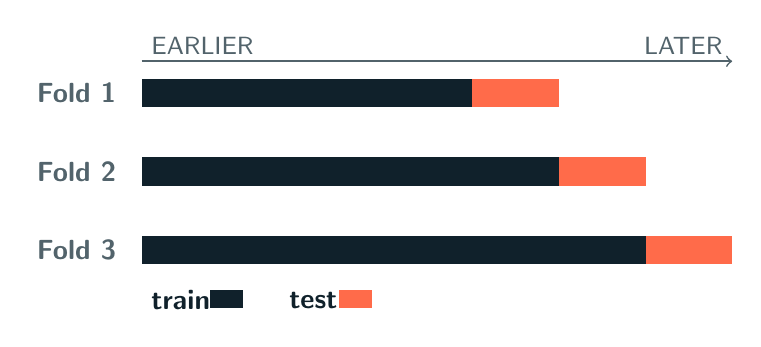
\begin{tikzpicture}[x=1cm,y=1cm]
        \foreach \y/\lab/\train/\test in {2.65/Fold 1/4.2/1.1,1.65/Fold 2/5.3/1.1,0.65/Fold 3/6.4/1.1}{
          \node[anchor=east,text=Slate,font=\bfseries\fontsize{10}{12}\selectfont] at (1.05,\y) {\lab};
          \fill[Ink] (1.25,\y-0.18) rectangle ++(\train,0.36);
          \fill[Coral] (1.25+\train,\y-0.18) rectangle ++(\test,0.36);
        }
        \node[anchor=west,text=Slate,font=\fontsize{9.5}{11}\selectfont] at (1.25,3.25) {EARLIER};
        \node[anchor=east,text=Slate,font=\fontsize{9.5}{11}\selectfont] at (8.75,3.25) {LATER};
        \draw[Slate,line width=0.6pt,->] (1.25,3.05) -- (8.75,3.05);
        \node[anchor=west,text=Ink,font=\fontsize{10}{12}\selectfont] at (1.25,0.02) {\textbf{train}};
        \fill[Ink] (2.12,-0.08) rectangle ++(0.42,0.22);
        \node[anchor=west,text=Ink,font=\fontsize{10}{12}\selectfont] at (3.0,0.02) {\textbf{test}};
        \fill[Coral] (3.75,-0.08) rectangle ++(0.42,0.22);
      \end{tikzpicture}
    \column{0.36\textwidth}
      \eyebrow{What this prevents}
      \vspace{0.18cm}
      \bodytext{Future leakage, optimistic backtests, and a single metric that masks failure.}
      \vspace{0.20cm}
      \eyebrow{Review together}
      \smalltext{Error \textbullet\ bias \textbullet\ interval coverage \textbullet\ stability}
  \end{columns}
  \vfill
  \smalltext{Demonstration project: the evaluation design is the evidence; no production impact is claimed.}
\end{frame}

% 06 --------------------------------------------------------------------------
\begin{frame}[t]
  \vspace{0.28cm}
  \slidetitle{Project 02 \textcolor{Coral}{/} Prioritization}{Risk is not the next-best action.}
  \vspace{0.28cm}
  \begin{columns}[T,onlytextwidth]
    \column{0.45\textwidth}
      \eyebrow{Question}
      \vspace{0.18cm}
      \bigline{Who should a limited team contact first?}
      \vspace{0.20cm}
      \smalltext{Risk alone ignores upside and whether an intervention is feasible.}
    \column{0.48\textwidth}
      \eyebrow{Priority logic}
      \vspace{0.18cm}
      {\fontsize{18}{21}\selectfont\bfseries\color{Ink}%
        priority $=$ risk $\times$ value\\
        $\times$ actionability\par}
      \vspace{0.22cm}
      \checkitem{Calibrate before ranking}
      \checkitem{Evaluate at team capacity}
      \checkitem{Translate reasons into review cues}
      \checkitem{Measure lift at the cutoff}
  \end{columns}
\end{frame}

% 07 --------------------------------------------------------------------------
\begin{frame}[t]
  \vspace{0.28cm}
  \slidetitle{Project 03 \textcolor{Coral}{/} Triage}{Automation needs an exit.}
  \vspace{0.24cm}
  \begin{columns}[T,onlytextwidth]
    \column{0.52\textwidth}
      \eyebrow{Routing policy}
      \vspace{0.20cm}
      \begin{tabular}{@{}>{\raggedright\arraybackslash}p{0.25\linewidth}>{\raggedright\arraybackslash}p{0.69\linewidth}@{}}
        \toprule
        \textbf{Signal} & \textbf{Action} \\
        \midrule
        High & Route automatically \\[0.15cm]
        Medium & Suggest; agent confirms \\[0.15cm]
        Low & Send to general queue \\
        \bottomrule
      \end{tabular}
      \vspace{0.18cm}
      \smalltext{Confidence is an operating control.}
    \column{0.41\textwidth}
      \eyebrow{Guardrails}
      \vspace{0.18cm}
      \checkitem{Macro and per-class recall}
      \checkitem{Abstention threshold}
      \checkitem{New-topic drift queue}
      \checkitem{Agent override captured}
      \checkitem{PII excluded from features}
  \end{columns}
\end{frame}

% 08 --------------------------------------------------------------------------
\begin{frame}[t]
  \vspace{0.28cm}
  \slidetitle{Delivery system}{One workflow, end to end.}
  \vspace{0.34cm}
  \begin{columns}[T,onlytextwidth]
    \column{0.19\textwidth}
      \step{\linewidth}{01}{Decision}{Frame choice and error cost.}
    \column{0.0125\textwidth}
      \mbox{}
    \column{0.19\textwidth}
      \step{\linewidth}{02}{Contract}{Set inputs and split.}
    \column{0.0125\textwidth}
      \mbox{}
    \column{0.19\textwidth}
      \step{\linewidth}{03}{Baseline}{Beat the simplest option.}
    \column{0.0125\textwidth}
      \mbox{}
    \column{0.19\textwidth}
      \step{\linewidth}{04}{Interface}{Deliver for use.}
    \column{0.0125\textwidth}
      \mbox{}
    \column{0.19\textwidth}
      \step{\linewidth}{05}{Monitor}{Watch data and action.}
  \end{columns}
  \vfill
  \begin{beamercolorbox}[wd=\textwidth,sep=0.22cm,left]{normal text}
    {\color{Leaf}\rule{0.8ex}{0.8ex}}\hspace{0.18cm}%
    {\fontsize{12.5}{15}\selectfont\bfseries The handoff is designed at the start, not appended at the end.}
  \end{beamercolorbox}
\end{frame}

% 09 --------------------------------------------------------------------------
\begin{frame}[t,fragile]
  \vspace{0.28cm}
  \slidetitle{Reproducibility}{Reviewable before impressive.}
  \vspace{0.22cm}
  \begin{columns}[T,onlytextwidth]
    \column{0.49\textwidth}
\begin{lstlisting}[style=portfolio]
project/
  data_contract.yml
  src/
    {features,train,evaluate}.py
  tests/
  reports/model_card.md
  Makefile
\end{lstlisting}
    \column{0.44\textwidth}
      \eyebrow{Review standard}
      \vspace{0.16cm}
      \checkitem{One command rebuilds outputs}
      \checkitem{Splits are deterministic}
      \checkitem{Assumptions live beside code}
      \checkitem{Metrics map to a decision}
      \checkitem{Limitations are explicit}
  \end{columns}
\end{frame}

% 10 --------------------------------------------------------------------------
\begin{frame}[t]
  \vspace{0.28cm}
  \slidetitle{Technical range}{Breadth delivers; depth protects.}
  \vspace{0.24cm}
  \begin{columns}[T,onlytextwidth]
    \column{0.57\textwidth}
      \eyebrow{Across the workflow}
      \vspace{0.18cm}
      \bodytext{SQL and data modeling \textcolor{Coral}{/} Python \textcolor{Coral}{/} experiment design \textcolor{Coral}{/} APIs \textcolor{Coral}{/} orchestration \textcolor{Coral}{/} dashboards \textcolor{Coral}{/} model monitoring}
      \vspace{0.28cm}
      {\color{Mist}\rule{\linewidth}{0.65pt}}
      \vspace{0.18cm}
      \smalltext{Tools change. The standard stays fixed: traceable inputs, honest evaluation, and a clear operating path.}
    \column{0.36\textwidth}
      \eyebrow{Deepest strengths}
      \vspace{0.18cm}
      \metric{01}{Evaluation design}
      \vspace{0.12cm}
      \metric{02}{Decision-focused modeling}
      \vspace{0.12cm}
      \metric{03}{Reproducible delivery}
  \end{columns}
\end{frame}

% 11 --------------------------------------------------------------------------
\begin{frame}[t]
  \vspace{0.28cm}
  \slidetitle{Team contribution}{Clarity at every handoff.}
  \vspace{0.28cm}
  \begin{columns}[T,onlytextwidth]
    \column{0.30\textwidth}
      {\fontsize{23}{25}\selectfont\bfseries\color{Coral}01\par}
      \vspace{0.10cm}
      {\fontsize{16}{18}\selectfont\bfseries Frame the decision\par}
      \vspace{0.10cm}
      \smalltext{Turn ambiguity into a measurable choice and an explicit error cost.}
    \column{0.04\textwidth}
      \centering{\color{Mist}\rule{0.8pt}{2.80cm}}
    \column{0.30\textwidth}
      {\fontsize{23}{25}\selectfont\bfseries\color{Coral}02\par}
      \vspace{0.10cm}
      {\fontsize{16}{18}\selectfont\bfseries Make evidence inspectable\par}
      \vspace{0.10cm}
      \smalltext{Build baselines and validation others can challenge and rerun.}
    \column{0.04\textwidth}
      \centering{\color{Mist}\rule{0.8pt}{2.80cm}}
    \column{0.30\textwidth}
      {\fontsize{23}{25}\selectfont\bfseries\color{Coral}03\par}
      \vspace{0.10cm}
      {\fontsize{16}{18}\selectfont\bfseries Design for adoption\par}
      \vspace{0.10cm}
      \smalltext{Ship thresholds, fallbacks, ownership, and monitoring.}
  \end{columns}
\end{frame}

% 12 --------------------------------------------------------------------------
\begin{frame}[plain]
  \begin{tikzpicture}[remember picture,overlay]
    \fill[Ink] (current page.south west) rectangle (current page.north east);
    \fill[Coral] (current page.south west) rectangle ([yshift=0.13cm]current page.south east);
    \fill[Mint] ([xshift=-0.18cm,yshift=-0.18cm]current page.north east) circle (1.05cm);
  \end{tikzpicture}
  \vspace{0.42cm}
  {\fontsize{10}{12}\selectfont\bfseries\color{Mint}\MakeUppercase{The next conversation}\par}
  \vfill
  \begin{minipage}{0.84\textwidth}
    \raggedright
    {\fontsize{34}{38}\selectfont\bfseries\color{White}%
      Bring a decision,\\a dataset, and a constraint.\par}
    \vspace{0.42cm}
    {\fontsize{18}{22}\selectfont\color{Mist}%
      I will bring a clear baseline, an honest test, and a path to use the result.\par}
  \end{minipage}
  \vfill
  {\fontsize{12}{14}\selectfont\bfseries\color{Mint}%
    PORTFOLIO REVIEW \hspace{0.25cm}\textcolor{Coral}{/}\hspace{0.25cm} CASE STUDY DEEP DIVE\par}
  \vspace{0.42cm}
\end{frame}

\end{document}
